\documentclass[border=10pt]{standalone}

\usepackage{tikz}
\usepackage{tikzsymbols}
\usetikzlibrary{calc,patterns,shapes.geometric}

\def\centerarc[#1](#2)(#3:#4:#5){\draw[#1] ($(#2)+({#5*cos(#3)},{#5*sin(#3)})$) arc (#3:#4:#5);}

\begin{document}
	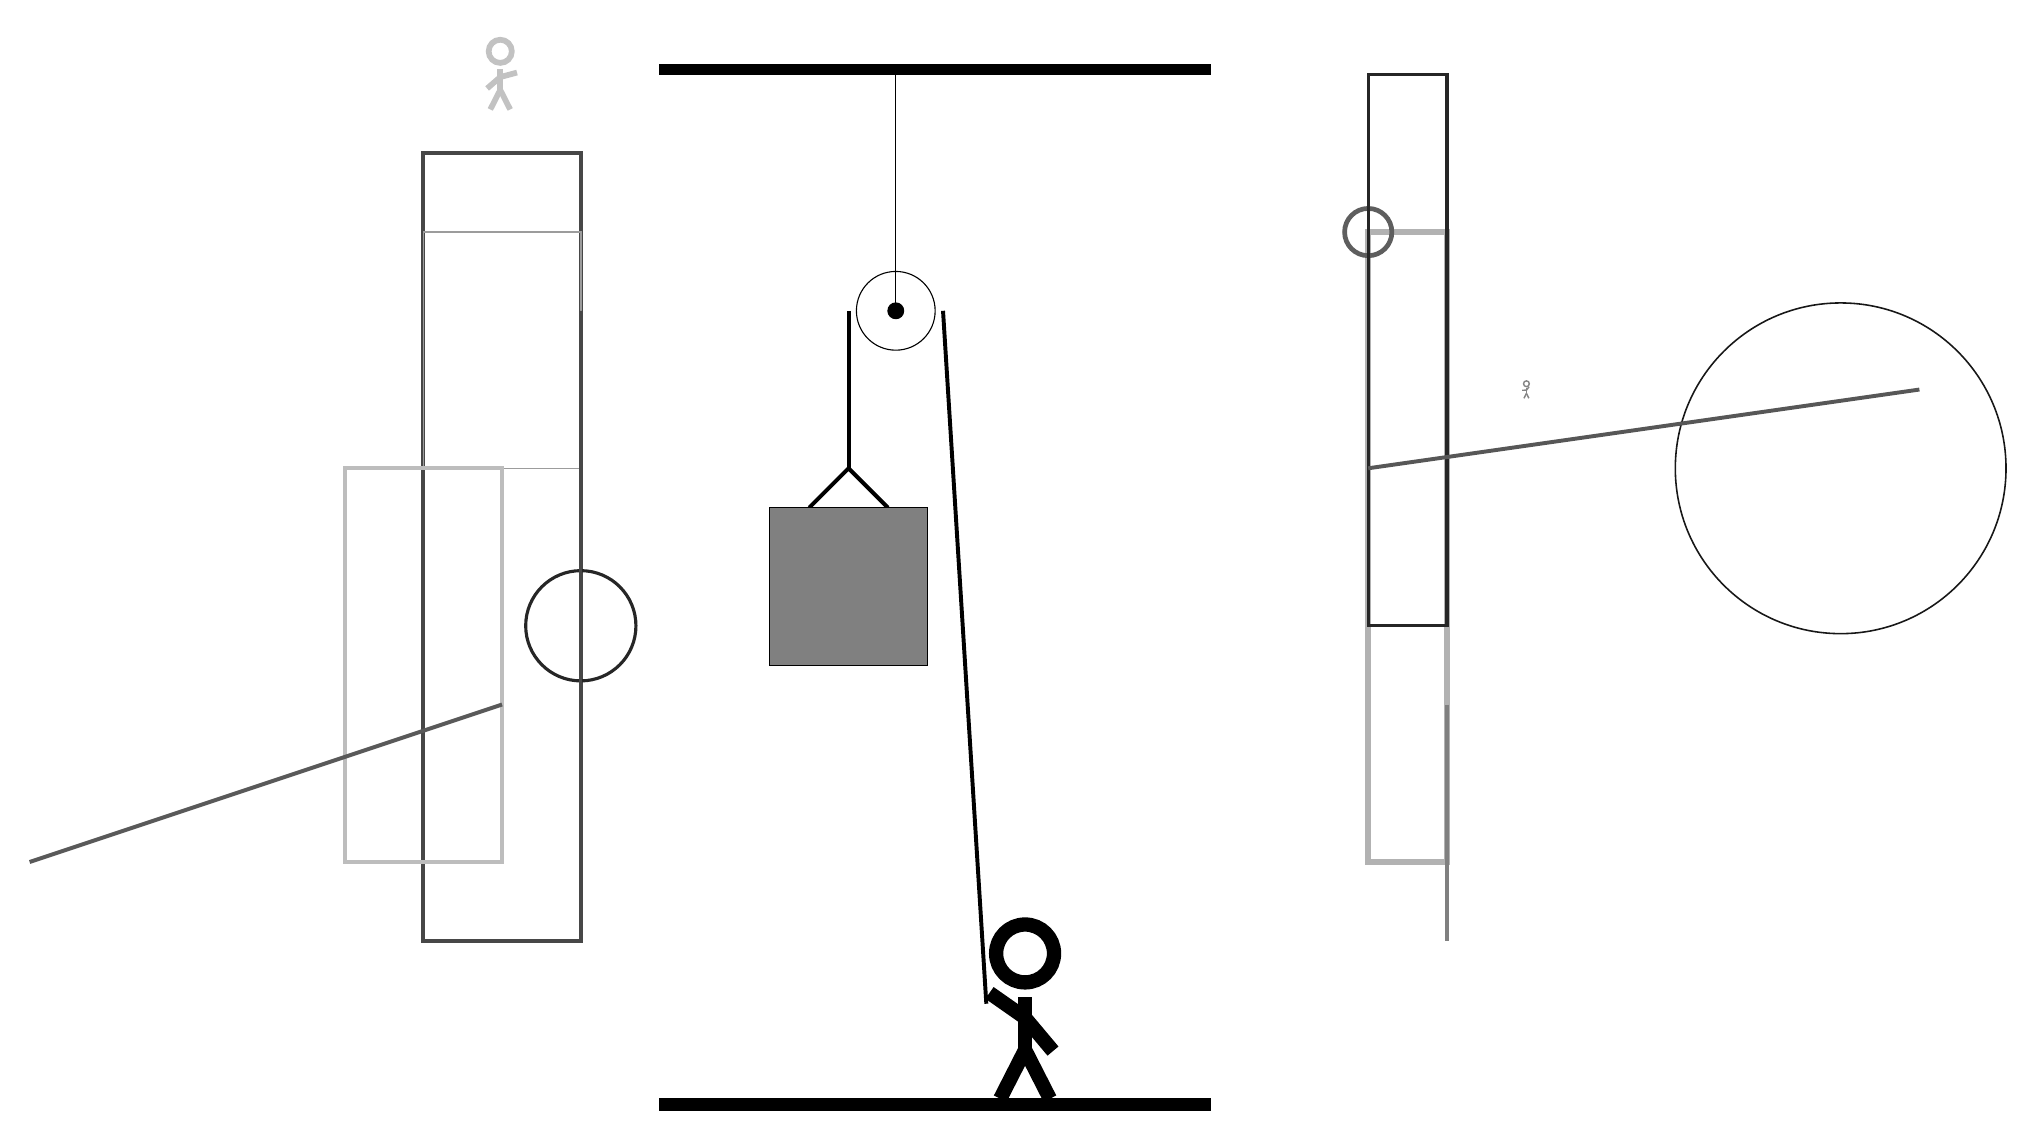
\begin{tikzpicture}
		%%%%% START %%%%%
		
		\draw[fill=black] (-2, 10) rectangle (5, 10.125);
		
		\draw[line width=0.7mm, color=black!30] (7, 8) rectangle (8, 0);
		
		\draw [line width=0.2mm, color=black!91](13, 5) circle (2.1);
		\draw[line width=0.5mm, color=black!72] (-3, 9) rectangle (-5, -1);
		\draw [line width=0.4mm, color=black!85](-3, 3) circle (0.7);
		\draw [line width=0.6mm, color=black!63](7, 8) circle (0.3);
		\draw[line width=0.2mm, color=black!39] (-3, 5) rectangle (-5, 8);
		\draw[line width=0.4mm, color=black!85] (7, 10) rectangle (8, 3);
		
		\draw[line width=0.5mm, color=black!50](8, 2) -- (8, -1);
		\node[line width=0.4mm, color=black!24] at (-4, 10) {\Strichmaxerl[4][41][15]};
		
		\draw[line width=0.5mm, color=black!26] (-4, 0) rectangle (-6, 5);
		
		\draw[line width=0.5mm, color=black!66](7, 5) -- (14, 6);
		\node[line width=0.5mm, color=black!48] at (9, 6) {\Strichmaxerl[1][1][52]};
		\draw[line width=0.4mm, color=black!72] (-3, 7) rectangle (-3, 1);
		
		\draw[line width=0.5mm, color=black!65](-4, 2) -- (-10, 0);
		
		\draw (1, 7) circle (0.5);
		\draw[fill=black] (1, 7) circle (0.1);
		\draw (1, 10) -- (1, 7);
		
		\draw[line width=0.5mm] (-0.1, 4.5) -- (0.4, 5.0) -- (0.9, 4.5);
		\draw[fill=black!50] (-0.6, 4.5) rectangle (1.4, 2.5);
		
		\draw[line width=0.5mm] (0.4, 7) -- (0.4, 5.0);
		\centerarc[line width=0.5mm](1, 7)(0:180:0.6);
		\draw[line width=0.5mm](1.6, 7) -- (2.15, -1.8);
		
		\node at (2.6, -1.9) {\Strichmaxerl[10][-35][-50]};
		
		\draw[fill=black] (-2, -3) rectangle (5, -3.15);
		
		%%%%% END %%%%%
	\end{tikzpicture}
\end{document}